\documentclass[t]{beamer}
\usetheme{Copenhagen}
\setbeamertemplate{headline}{} % remove toc from headers
\beamertemplatenavigationsymbolsempty

\usepackage{amsmath, tikz, bm, tkz-euclide}
\usetkzobj{all}

\title{Trig Functions of Any Angle}
\author{}
\date{}

\AtBeginSection[]
{
  \begin{frame}
    \frametitle{Objectives}
    \tableofcontents[currentsection]
  \end{frame}
}

\begin{document}

\begin{frame} 
\maketitle
\end{frame}

\begin{frame}{From Right Triangle Trig to the Coordinate Plane}
In this section, adjacent, opposite and hypotenuse
\begin{center}
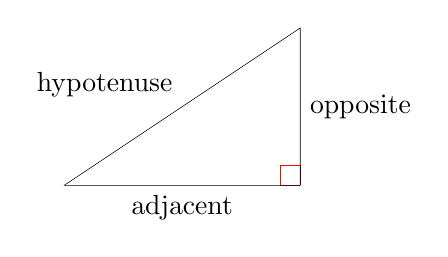
\begin{tikzpicture}
    \tkzDefPoints{0/0/A, 3/0/C, 3/2/B}
    \tkzMarkRightAngle[color=red](A,C,B)
    \tkzDrawPolygon(A,B,C)
    \tkzLabelSegment[below](A,C){adjacent}
    \tkzLabelSegment[right](B,C){opposite}
    \tkzLabelSegment[above left](A,B){hypotenuse}
\end{tikzpicture}
\end{center}
\end{frame}

\begin{frame}{From Right Triangle Trig to the Coordinate Plane}
become
\begin{center}
    \begin{tikzpicture}
    \draw [<->, >=stealth] (-3,0) -- (3,0) node [right] {$x$};
    \draw [<->, >=stealth] (0,-3) -- (0,3) node [right] {$y$};
    \draw [color=red] (2.5,0) rectangle (2.25,0.25);
    \draw (0,0) -- (2.5,0) -- (2.5,2) -- cycle;
    \node at (1.25,0) [below] {$\bm{x}$};
    \node at (2.5,1) [right] {$\bm{y}$};
    \node at (1.25,1) [above] {$\bm{r}$};
    \end{tikzpicture}
\end{center}
\end{frame}

\begin{frame}{From Right Triangle Trig to the Coordinate Plane}
where $r$ represents the radius of the circle shown below.

\begin{center}
    \begin{tikzpicture}
    \draw [<->, >=stealth] (-3,0) -- (3,0) node [right] {$x$};
    \draw [<->, >=stealth] (0,-3) -- (0,3) node [right] {$y$};
    \draw [color=red] (2.5,0) rectangle (2.25,0.25);
    \draw (0,0) -- (2.5,0) -- (2.5,2) -- cycle;
    \node at (1.25,0) [below] {$\bm{x}$};
    \node at (2.5,1) [right] {$\bm{y}$};
    \node at (1.25,1) [above] {$\bm{r}$};
    \draw [dashed] (0,0) circle (3.2cm);
    \node at (0,0) [below left] {$A$};
    \end{tikzpicture}
\end{center}
\end{frame}

\begin{frame}{From Right Triangle Trig to the Coordinate Plane}
The biggest difference between this section and the last is that in this section, trig ratios can be positive, negative, zero, or undefined, since $x$ and $y$ can each be positive, negative, or zero. 
\end{frame}

\section{Calculate the 6 Trig Ratios for a Point in the Coordinate Plane}

\begin{frame}{The 6 Trig Ratios}
In the coordinate plane, the six trig ratios become \newline\\
\begin{center}
    \begin{tabular}{c|c}
        $\sin A = \dfrac{y}{r}$  &   \onslide<2->{$\csc A = \dfrac{r}{y}$}    \\[0.35in]
        $\cos A = \dfrac{x}{r}$ &   \onslide<2->{$\sec A = \dfrac{r}{x}$}   \\[0.35in]
        $\tan A = \dfrac{y}{x}$ &   \onslide<2->{$\cot A = \dfrac{x}{y}$}   \\
    \end{tabular}
\end{center}
\end{frame}

\begin{frame}{Example 1a}
For the given point, find the exact values of the 6 trig functions for the angle drawn in standard form.   \newline\\
(a)     \quad $(3,-4)$
\begin{align*}
\onslide<2->{3^2 + 4^2 &= r^2}	\\[8pt]
\onslide<3->{r &= \sqrt{25} = 5} \\
\end{align*}
\begin{tabular}{p{0.4\textwidth}p{0.4\textwidth}}
\onslide<4->{$\sin A = \frac{-4}{5}$}	&	\onslide<7->{$\csc A = \frac{5}{-4}$}	\\[8pt]
\onslide<5->{$\cos A = \frac{3}{5}$}	&	\onslide<8->{$\sec A = \frac{5}{3}$}	\\[8pt]
\onslide<6->{$\tan A = \frac{-4}{3}$}	&	\onslide<9->{$\cot A = \frac{3}{-4}$}	\\
\end{tabular}
\end{frame}

\begin{frame}{Example 1b}
(b)	\quad $(-8,-15)$
\begin{align*}
\onslide<2->{8^2 + 15^2 &= r^2}	\\[8pt]
\onslide<3->{r &= \sqrt{289} = 17} \\
\end{align*}
\begin{tabular}{p{0.4\textwidth}p{0.4\textwidth}}
\onslide<4->{$\sin A = \frac{-15}{17}$}					&	\onslide<7->{$\csc A = \frac{17}{-15}$}	\\[8pt]
\onslide<5->{$\cos A = \frac{-8}{17}$}					&	\onslide<8->{$\sec A = \frac{17}{-8}$}	\\[8pt]
\onslide<6->{$\tan A = \frac{-15}{-8} = \frac{15}{8}$}	&	\onslide<9->{$\cot A = \frac{8}{15}$}	\\
\end{tabular}
\end{frame}

\begin{frame}{Example 1c}
(c)	\quad $(-1,5)$
\begin{align*}
\onslide<2->{1^2 + 5^2 &= r^2}	\\[8pt]
\onslide<3->{r &= \sqrt{26}} \\
\end{align*}
\begin{tabular}{p{0.4\textwidth}p{0.4\textwidth}}
\onslide<4->{$\sin A = \frac{5}{\sqrt{26}} = \frac{5\sqrt{26}}{26}$}	&	\onslide<7->{$\csc A = \frac{\sqrt{26}}{5}$}	\\[8pt]
\onslide<5->{$\cos A = \frac{-1}{\sqrt{26}} = \frac{-\sqrt{26}}{26}$}	&	\onslide<8->{$\sec A = \frac{\sqrt{26}}{-1} = -\sqrt{26}$}	\\[8pt]
\onslide<6->{$\tan A = \frac{5}{-1} = -5$}	&	\onslide<9->{$\cot A = \frac{-1}{5}$}	\\
\end{tabular}
\end{frame}


\section{Find the Exact Values of the Trig Ratios of Special Angles in the Coordinate Plane}

\begin{frame}
If we put a 45-45-90 triangle in the second quadrant of the coordinate plane, it would resemble the following:

\begin{center}
    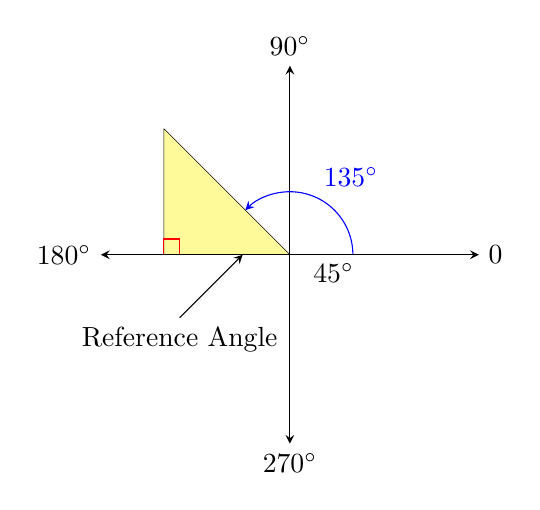
\begin{tikzpicture}[scale=0.8]
    \tkzDefPoints{0/0/A, -2/0/C, -2/2/B}
    \tkzDrawPolygon[fill=yellow!40](A,B,C)
    \tkzMarkRightAngle[color=red](B,C,A)
    \draw [<->, >=stealth] (-3,0) node [left] {$180^\circ$} -- (3,0) node [right] {$0$};
    \draw [<->, >=stealth] (0,-3) node [below] {$270^\circ$} -- (0,3) node [above] {$90^\circ$};
    \tkzLabelAngle[pos=0.75](C,A,B){$45^\circ$}
    \onslide<2->{\draw [->, >=stealth, color=blue] (0:1) arc (0:135:1) node [midway, above right, color=blue] {$135^\circ$};}
    \onslide<4->{\draw[->, >=stealth] (-1.75,-1) node [below] {Reference Angle} -- (-0.75,0);}
    \end{tikzpicture}
\end{center}
\pause

The hypotenuse, $r$, would have rotated $180^\circ - 45^\circ = 135^\circ$.  
\end{frame}

\begin{frame} 
In the second quadrant, $x$-coordinates are negative and $y$-coordinates are positive ($r$ is always positive). Thus, the values would be

\begin{center}
    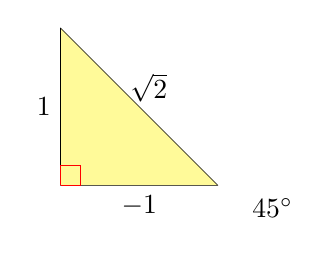
\begin{tikzpicture}
    \tkzDefPoints{0/0/A, -2/0/C, -2/2/B}
    \tkzDrawPolygon[fill=yellow!40](A,B,C)
    \tkzMarkRightAngle[color=red](B,C,A)
    \tkzLabelAngle[pos=0.75](C,A,B){$45^\circ$}
    \node at (-1,0) [below] {$-1$};
    \node at (-2,1) [left] {$1$};
    \node at (135:1.75) [right] {$\sqrt{2}$};
    \end{tikzpicture}
\end{center}
\pause
So $\sin 135^\circ = \frac{\sqrt{2}}{2}$, $\cos 135^\circ = -\frac{\sqrt{2}}{2}$, and $\tan 135^\circ = -1$.
\end{frame}

\begin{frame}{Example 2a}
Find the exact values of the 6 trig functions for each of the following.	\newline\\
(a)	\quad $135^\circ = \frac{3\pi}{4}$	\newline\\
\begin{minipage}{0.25\textwidth}
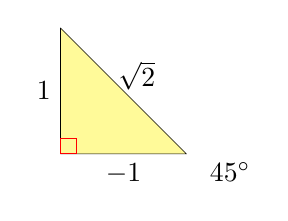
\begin{tikzpicture}[scale=0.8]
    \tkzDefPoints{0/0/A, -2/0/C, -2/2/B}
    \tkzDrawPolygon[fill=yellow!40](A,B,C)
    \tkzMarkRightAngle[color=red](B,C,A)
    \onslide<1->{\tkzLabelAngle[pos=0.75](C,A,B){$45^\circ$}}
    \node at (-1,0) [below] {$-1$};
    \node at (-2,1) [left] {$1$};
    \node at (135:1.75) [right] {$\sqrt{2}$};
    \end{tikzpicture}
\end{minipage}
\begin{minipage}{0.65\textwidth}
\begin{tabular}{p{0.43\textwidth}p{0.53\textwidth}}
\onslide<1->{$\sin 135^\circ = \frac{\sqrt{2}}{2}$}		&	\onslide<2->{$\csc 135^\circ = \frac{\sqrt{2}}{1} = \sqrt{2}$}	\\[11pt]
\onslide<1->{$\cos 135^\circ = -\frac{\sqrt{2}}{2}$}	&	\onslide<3->{$\sec 135^\circ = \frac{\sqrt{2}}{-1} = -\sqrt{2}$}	\\[11pt]
\onslide<1->{$\tan 135^\circ = -1$}						&	\onslide<4->{$\cot 135^\circ = -1$}	\\
\end{tabular}
\end{minipage}
\end{frame}

\begin{frame}{Example 2b}
(b)	\quad $225^\circ = \frac{5\pi}{4}$	\newline\\
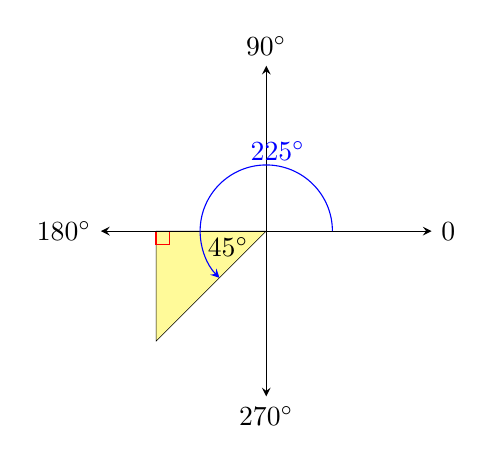
\begin{tikzpicture}[scale=0.7]
    \tkzDefPoints{0/0/A, -2/0/C, -2/-2/B}
    \tkzDrawPolygon[fill=yellow!40](A,B,C)
    \tkzMarkRightAngle[color=red](B,C,A)
    \draw [<->, >=stealth] (-3,0) node [left] {$180^\circ$} -- (3,0) node [right] {$0$};
    \draw [<->, >=stealth] (0,-3) node [below] {$270^\circ$} -- (0,3) node [above] {$90^\circ$};
    \onslide<2->{\tkzLabelAngle[pos=-0.75](B,A,C){$45^\circ$}}
    \draw [->, >=stealth, color=blue] (0:1.2) arc (0:225:1.2) node [midway, above right, color=blue] {$225^\circ$};
\end{tikzpicture}
\end{frame}

\begin{frame}{Example 2b}
\begin{center}
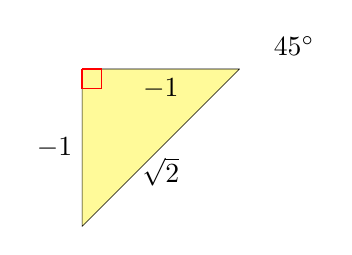
\begin{tikzpicture}
    \tkzDefPoints{0/0/A, -2/0/C, -2/-2/B}
    \tkzDrawPolygon[fill=yellow!40](A,B,C)
    \tkzMarkRightAngle[color=red](B,C,A)
    \tkzLabelAngle[pos=-0.75](C,A,B){$45^\circ$}
    \tkzLabelSegment[midway](A,C){$-1$}
    \tkzLabelSegment[midway, left](C,B){$-1$}
    \tkzLabelSegment[below](A,B){$\sqrt{2}$}
\end{tikzpicture} 
\end{center}
\begin{tabular}{p{0.5\textwidth}p{0.5\textwidth}}
\onslide<2->{$\sin 225^\circ = \frac{-1}{\sqrt{2}} = -\frac{\sqrt{2}}{2}$}	&	\onslide<5->{$\csc 225^\circ = \frac{\sqrt{2}}{-1} = -\sqrt{2}$}	\\[11pt]
\onslide<3->{$\cos 225^\circ = \frac{-1}{\sqrt{2}} = -\frac{\sqrt{2}}{2}$}	&	\onslide<6->{$\sec 225^\circ = \frac{\sqrt{2}}{-1} = -\sqrt{2}$}	\\[11pt]
\onslide<4->{$\tan 225^\circ = \frac{-1}{-1} = 1$}							&	\onslide<7->{$\cot 225^\circ = \frac{-1}{-1} = 1$}	\\
\end{tabular}
\end{frame}

\begin{frame}{Example 2c}
(c) \quad $315^\circ = \frac{7\pi}{4}$	\newline\\
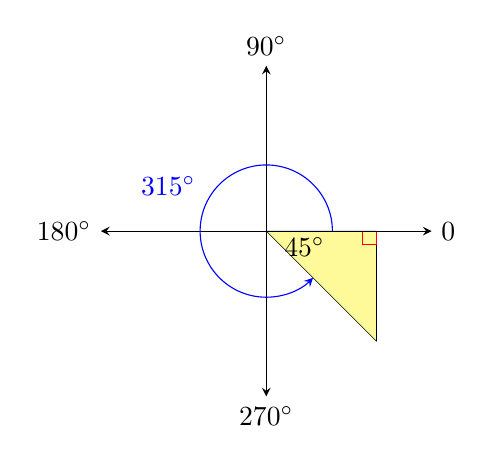
\begin{tikzpicture}[scale=0.7]
    \tkzDefPoints{0/0/A, 2/0/C, 2/-2/B}
    \tkzDrawPolygon[fill=yellow!40](A,B,C)
    \tkzMarkRightAngle[color=red](B,C,A)
    \draw [<->, >=stealth] (-3,0) node [left] {$180^\circ$} -- (3,0) node [right] {$0$};
    \draw [<->, >=stealth] (0,-3) node [below] {$270^\circ$} -- (0,3) node [above] {$90^\circ$};
    \onslide<2->{\tkzLabelAngle[pos=0.75](B,A,C){$45^\circ$}}
    \draw [->, >=stealth, color=blue] (0:1.2) arc (0:315:1.2) node [midway, above left, color=blue] {$315^\circ$};
\end{tikzpicture}
\end{frame}

\begin{frame}{Example 2c}
\begin{center}
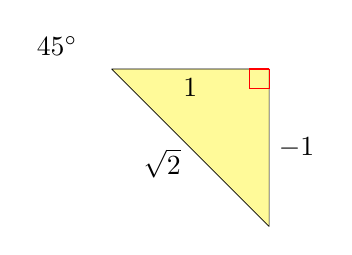
\begin{tikzpicture}
    \tkzDefPoints{0/0/A, 2/0/C, 2/-2/B}
    \tkzDrawPolygon[fill=yellow!40](A,B,C)
    \tkzMarkRightAngle[color=red](B,C,A)
    \tkzLabelAngle[pos=0.75](C,A,B){$45^\circ$}
    \tkzLabelSegment[midway](A,C){$1$}
    \tkzLabelSegment[midway, right](C,B){$-1$}
    \tkzLabelSegment[below, left, yshift=-0.2cm](A,B){$\sqrt{2}$}
\end{tikzpicture} 
\end{center}
\begin{tabular}{p{0.5\textwidth}p{0.5\textwidth}}
\onslide<2->{$\sin 315^\circ = \frac{-1}{\sqrt{2}} = -\frac{\sqrt{2}}{2}$}	&	\onslide<5->{$\csc 315^\circ = \frac{\sqrt{2}}{-1} = -\sqrt{2}$}	\\[11pt]
\onslide<3->{$\cos 315^\circ = \frac{1}{\sqrt{2}} = \frac{\sqrt{2}}{2}$}	&	\onslide<6->{$\sec 315^\circ = \frac{\sqrt{2}}{1} = \sqrt{2}$}	\\[11pt]
\onslide<4->{$\tan 315^\circ = \frac{-1}{1} = -1$}							&	\onslide<7->{$\cot 315^\circ = \frac{1}{-1} = -1$}	\\
\end{tabular}
\end{frame}

\begin{frame}{Example 2d}
(d) \quad $120^\circ = \frac{2\pi}{3}$	\newline\\
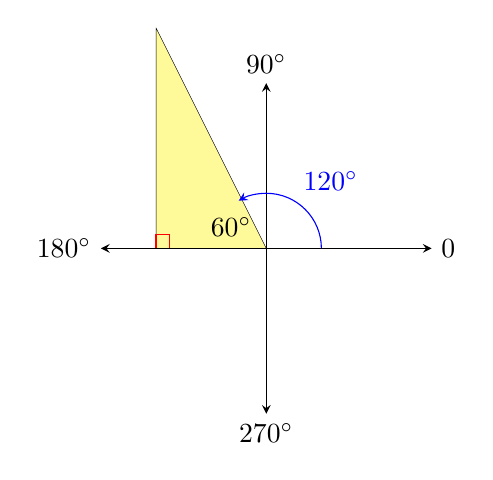
\begin{tikzpicture}[scale=0.7]
    \tkzDefPoints{0/0/A, -2/0/C, -2/4/B}
    \tkzDrawPolygon[fill=yellow!40](A,B,C)
    \tkzMarkRightAngle[color=red](B,C,A)
    \draw [<->, >=stealth] (-3,0) node [left] {$180^\circ$} -- (3,0) node [right] {$0$};
    \draw [<->, >=stealth] (0,-3) node [below] {$270^\circ$} -- (0,3) node [above] {$90^\circ$};
    \onslide<2->{\tkzLabelAngle[pos=0.75](B,A,C){$60^\circ$}}
    \draw [->, >=stealth, color=blue] (0:1) arc (0:120:1) node [midway, above right, color=blue] {$120^\circ$};
\end{tikzpicture}
\end{frame}

\begin{frame}{Example 2d}
\begin{center}
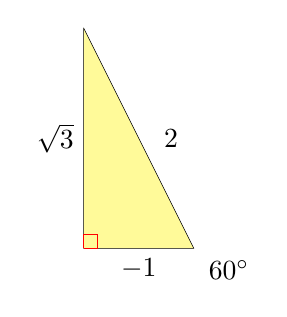
\begin{tikzpicture}[scale=0.7]
    \tkzDefPoints{0/0/A, -2/0/C, -2/4/B}
    \tkzDrawPolygon[fill=yellow!40](A,B,C)
    \tkzMarkRightAngle[color=red](B,C,A)
    \tkzLabelAngle[pos=0.75](C,A,B){$60^\circ$}
    \tkzLabelSegment[midway,below](A,C){$-1$}
    \tkzLabelSegment[midway, left](C,B){$\sqrt{3}$}
    \tkzLabelSegment[right, xshift=0.2cm](A,B){$2$}
\end{tikzpicture} 
\end{center}
\begin{tabular}{p{0.5\textwidth}p{0.5\textwidth}}
\onslide<2->{$\sin 120^\circ = \frac{\sqrt{3}}{2}$}					&	\onslide<5->{$\csc 120^\circ = \frac{2}{\sqrt{3}} = \frac{2\sqrt{3}}{3}$}	\\[11pt]
\onslide<3->{$\cos 120^\circ = \frac{-1}{2}$}						&	\onslide<6->{$\sec 120^\circ = \frac{2}{-1} = -2$}	\\[11pt]
\onslide<4->{$\tan 120^\circ = \frac{\sqrt{3}}{-1} = -\sqrt{3}$}	&	\onslide<7->{$\cot 120^\circ = \frac{-1}{\sqrt{3}} = -\frac{\sqrt{3}}{3}$}	\\
\end{tabular}
\end{frame}

\begin{frame}{Example 2e}
(e) \quad $150^\circ = \frac{5\pi}{6}$	\newline\\
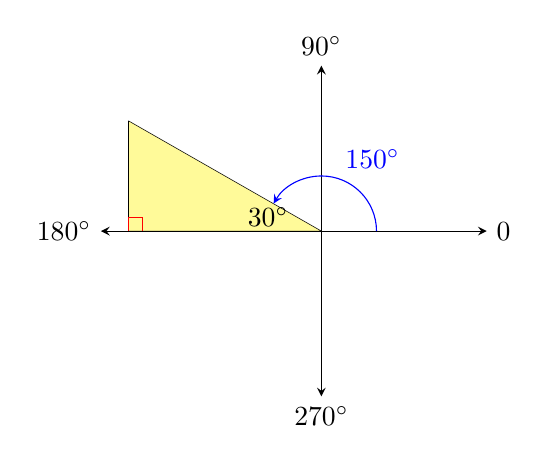
\begin{tikzpicture}[scale=0.7]
    \tkzDefPoints{0/0/A, -3.5/0/C, -3.5/2/B}
    \tkzDrawPolygon[fill=yellow!40](A,B,C)
    \tkzMarkRightAngle[color=red](B,C,A)
    \draw [<->, >=stealth] (-4,0) node [left] {$180^\circ$} -- (3,0) node [right] {$0$};
    \draw [<->, >=stealth] (0,-3) node [below] {$270^\circ$} -- (0,3) node [above] {$90^\circ$};
    \onslide<2->{\tkzLabelAngle[pos=1](B,A,C){$30^\circ$}}
    \draw [->, >=stealth, color=blue] (0:1) arc (0:150:1) node [midway, above right, color=blue] {$150^\circ$};
\end{tikzpicture}
\end{frame}

\begin{frame}{Example 2e}
\begin{center}
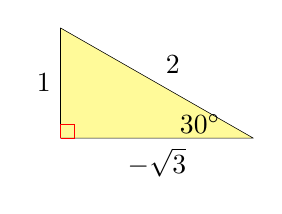
\begin{tikzpicture}[scale=0.7]
    \tkzDefPoints{0/0/A, -3.5/0/C, -3.5/2/B}
    \tkzDrawPolygon[fill=yellow!40](A,B,C)
    \tkzMarkRightAngle[color=red](B,C,A)
    \tkzLabelSegment[below](A,C){$-\sqrt{3}$}
    \tkzLabelSegment[left](C,B){1}
    \tkzLabelSegment[above, xshift = 0.2cm](A,B){2}
    \tkzLabelAngle[pos=1](B,A,C){$30^\circ$}
\end{tikzpicture}
\end{center}
\begin{tabular}{p{0.5\textwidth}p{0.5\textwidth}}
\onslide<2->{$\sin 150^\circ = \frac{1}{2}$}					&	\onslide<5->{$\csc 150^\circ = \frac{2}{1} = 2$}	\\[11pt]
\onslide<3->{$\cos 150^\circ = \frac{-\sqrt{3}}{2}$}			&	\onslide<6->{$\sec 150^\circ = \frac{2}{-\sqrt{3}} = -\frac{2\sqrt{3}}{3}$}	\\[11pt]
\onslide<4->{$\tan 150^\circ = \frac{1}{-\sqrt{3}} = -\frac{\sqrt{3}}{3}$}	&	\onslide<7->{$\cot 150^\circ = \frac{-\sqrt{3}}{1} = -\sqrt{3}$}	\\
\end{tabular}
\end{frame}

\begin{frame}{Example 2f}
(a) \quad $210^\circ = \frac{7\pi}{6}$	\newline\\
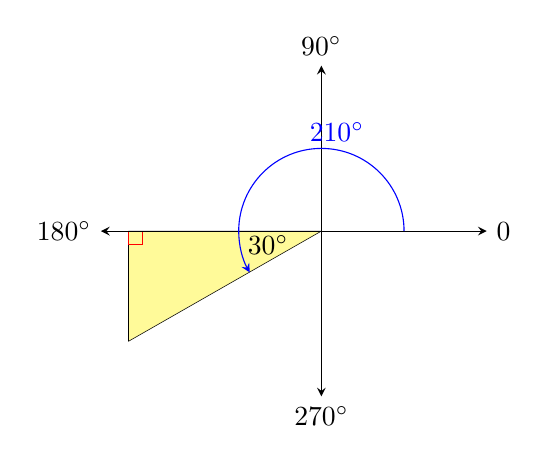
\begin{tikzpicture}[scale=0.7]
    \tkzDefPoints{0/0/A, -3.5/0/C, -3.5/-2/B}
    \tkzDrawPolygon[fill=yellow!40](A,B,C)
    \tkzMarkRightAngle[color=red](B,C,A)
    \draw [<->, >=stealth] (-4,0) node [left] {$180^\circ$} -- (3,0) node [right] {$0$};
    \draw [<->, >=stealth] (0,-3) node [below] {$270^\circ$} -- (0,3) node [above] {$90^\circ$};
    \onslide<2->{\tkzLabelAngle[pos=-1](B,A,C){$30^\circ$}}
    \draw [->, >=stealth, color=blue] (0:1.5) arc (0:210:1.5) node [midway, above right, color=blue] {$210^\circ$};
\end{tikzpicture}
\end{frame}

\begin{frame}{Example 2f}
\begin{center}
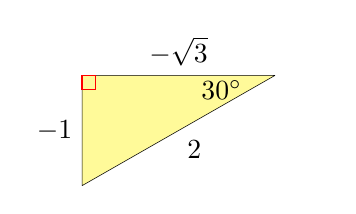
\begin{tikzpicture}[scale=0.7]
    \tkzDefPoints{0/0/A, -3.5/0/C, -3.5/-2/B}
    \tkzDrawPolygon[fill=yellow!40](A,B,C)
    \tkzMarkRightAngle[color=red](B,C,A)
    \tkzLabelSegment[above](A,C){$-\sqrt{3}$}
    \tkzLabelSegment[left](C,B){$-1$}
    \tkzLabelSegment[below, xshift = 0.2cm](A,B){2}
    \tkzLabelAngle[pos=-1](B,A,C){$30^\circ$}
\end{tikzpicture}
\end{center}
\begin{tabular}{p{0.5\textwidth}p{0.5\textwidth}}
\onslide<2->{$\sin 210^\circ = \frac{-1}{2}$}					&	\onslide<5->{$\csc 210^\circ = \frac{2}{-1} = -2$}	\\[11pt]
\onslide<3->{$\cos 210^\circ = \frac{-\sqrt{3}}{2}$}			&	\onslide<6->{$\sec 210^\circ = \frac{2}{-\sqrt{3}} = -\frac{2\sqrt{3}}{3}$}	\\[11pt]
\onslide<4->{$\tan 210^\circ = \frac{-1}{-\sqrt{3}} = \frac{\sqrt{3}}{3}$}	&	\onslide<7->{$\cot 210^\circ = \frac{-\sqrt{3}}{-1} = \sqrt{3}$}	\\
\end{tabular}
\end{frame}

\begin{frame}{Quadrantal Angles}
A \alert{quadrantal angle} is an angle whose terminal side lies on an axis.  \newline\\  \pause


Finding the values of the trig functions for quadrantal angles can be found by using any point on the axes.
\end{frame}

\begin{frame}{Quadrantal Angles}
For simplicity, we will use combinations of 0s and 1s. Below is the point we will use for $0^\circ$.
\begin{center}
    \begin{tikzpicture}[scale=0.8]
    \draw [<->, >=stealth] (-3,0) -- (3,0) node [right] {$0$};
    \draw [<->, >=stealth] (0,-3) -- (0,3);
    \draw [fill=black] (2,0) circle (2pt) node [below] {$(1,0)$};
    \draw [->, >=latex, line width = 1.5, color=blue] (0,0) -- node [above] {$r=1$} (2,0);
    \node at (0,3) [right] {$90^\circ$};
    \node at (-3,0) [left] {$180^\circ$};
    \node at (0,-3) [right] {$270^\circ$};
    \end{tikzpicture}
\end{center}
\end{frame}

\begin{frame}{Quadrantal Angles}
So, for $0^\circ$, we have $x=1, \, y=0, \, \text{and } r=1$. Thus  \newline\\ 

\begin{center}
\begin{tabular}{p{0.3\textwidth}p{0.5\textwidth}}
    \onslide<2->{$\sin 0 = \frac{0}{1} = 0$}  &
    \onslide<5->{$\csc 0 = \frac{1}{0} = \text{undefined}$}  \\[18pt]
    \onslide<3->{$\cos 0 = \frac{1}{1} = 1$}  &
    \onslide<6->{$\sec 0 = \frac{1}{1} = 1$}  \\[18pt]
    \onslide<4->{$\tan 0 = \frac{0}{1} = 0$}  &
    \onslide<7->{$\cot 0 = \frac{1}{0} = \text{undefined}$}   \\
\end{tabular}
\end{center}
\end{frame}

\begin{frame}{Example 3a}
Find the exact values of each of the 6 trig functions for the following angles.   \newline\\
(a) \quad $90^\circ = \frac{\pi}{2}$    \newline\\  \pause
\begin{minipage}{0.5\textwidth}
\begin{tikzpicture}[scale=0.7]
    \draw [<->, >=stealth] (-3,0) -- (3,0) node [right] {$0$};
    \draw [<->, >=stealth] (0,-3) -- (0,3);
    \draw [fill=black] (0,2) circle (2pt) node [right] {$(0,1)$};
    \draw [->, >=latex, line width = 1.5, color=blue] (0,0) -- node [right] {$r=1$} (0,2);
    \node at (0,3) [right] {$90^\circ$};
    \node at (-3,0) [left] {$180^\circ$};
    \node at (0,-3) [right] {$270^\circ$};
\end{tikzpicture}
\end{minipage}
\hspace{0.35cm}
\begin{minipage}{0.3\textwidth}
\begin{align*}
    \onslide<3->{\sin 90^\circ &= \frac{1}{1} = 1} \\[18pt]
    \onslide<4->{\cos 90^\circ &= \frac{0}{1} = 0} \\[18pt]
    \onslide<5->{\tan 90^\circ &= \frac{1}{0} = \text{undefined}} \\
\end{align*}
\end{minipage}
\end{frame}

\begin{frame}{Example 3a}
\begin{minipage}{0.5\textwidth}
\begin{tikzpicture}[scale=0.7]
    \draw [<->, >=stealth] (-3,0) -- (3,0) node [right] {$0$};
    \draw [<->, >=stealth] (0,-3) -- (0,3);
    \draw [fill=black] (0,2) circle (2pt) node [right] {$(0,1)$};
    \draw [->, >=latex, line width = 1.5, color=blue] (0,0) -- node [right] {$r=1$} (0,2);
    \node at (0,3) [right] {$90^\circ$};
    \node at (-3,0) [left] {$180^\circ$};
    \node at (0,-3) [right] {$270^\circ$};
\end{tikzpicture}
\end{minipage}
\hspace{0.35cm}
\begin{minipage}{0.3\textwidth}
\begin{align*}
    \onslide<2->{\csc 90^\circ &= \frac{1}{1} = 1} \\[18pt]
    \onslide<3->{\sec 90^\circ &= \frac{1}{0} = \text{undefined}} \\[18pt]
    \onslide<4->{\cot 90^\circ &= \frac{0}{1} = 0} \\
\end{align*}
\end{minipage}
\end{frame}

\begin{frame}{Example 3b}
    (b) \quad $180^\circ = \pi$    \newline\\  \pause
\begin{minipage}{0.5\textwidth}
\begin{tikzpicture}[scale=0.7]
    \draw [<->, >=stealth] (-3,0) -- (3,0) node [right] {$0$};
    \draw [<->, >=stealth] (0,-3) -- (0,3);
    \draw [fill=black] (-2,0) circle (2pt) node [below] {$(-1,0)$};
    \draw [->, >=latex, line width = 1.5, color=blue] (0,0) -- node [above] {$r=1$} (-2,0);
    \node at (0,3) [right] {$90^\circ$};
    \node at (-3,0) [left] {$180^\circ$};
    \node at (0,-3) [right] {$270^\circ$};
\end{tikzpicture}
\end{minipage}
\hspace{0.35cm}
\begin{minipage}{0.3\textwidth}
\begin{align*}
    \onslide<3->{\sin 180^\circ &= \frac{0}{1} = 0} \\[18pt]
    \onslide<4->{\cos 180^\circ &= \frac{-1}{1} = -1} \\[18pt]
    \onslide<5->{\tan 180^\circ &= \frac{0}{-1} = 0} \\
\end{align*}
\end{minipage}
\end{frame}

\begin{frame}{Example 3b}
\begin{minipage}{0.5\textwidth}
\begin{tikzpicture}[scale=0.7]
    \draw [<->, >=stealth] (-3,0) -- (3,0) node [right] {$0$};
    \draw [<->, >=stealth] (0,-3) -- (0,3);
    \draw [fill=black] (-2,0) circle (2pt) node [below] {$(-1,0)$};
    \draw [->, >=latex, line width = 1.5, color=blue] (0,0) -- node [above] {$r=1$} (-2,0);
    \node at (0,3) [right] {$90^\circ$};
    \node at (-3,0) [left] {$180^\circ$};
    \node at (0,-3) [right] {$270^\circ$};
\end{tikzpicture}
\end{minipage}
\hspace{0.35cm}
\begin{minipage}{0.3\textwidth}
\begin{align*}
    \onslide<2->{\csc 180^\circ &= \frac{1}{0} = \text{undefined}} \\[18pt]
    \onslide<3->{\sec 180^\circ &= \frac{1}{-1} = -1} \\[18pt]
    \onslide<4->{\cot 180^\circ &= \frac{-1}{0} = \text{undefined}} \\
\end{align*}
\end{minipage}
\end{frame}

\begin{frame}{Example 3c}
(c) \quad $270^\circ = \frac{3\pi}{2}$    \newline\\  \pause
\begin{minipage}{0.5\textwidth}
\begin{tikzpicture}[scale=0.7]
    \draw [<->, >=stealth] (-3,0) -- (3,0) node [right] {$0$};
    \draw [<->, >=stealth] (0,-3) -- (0,3);
    \draw [fill=black] (0,-2) circle (2pt) node [right] {$(0,-1)$};
    \draw [->, >=latex, line width = 1.5, color=blue] (0,0) -- node [left] {$r=1$} (0,-2);
    \node at (0,3) [right] {$90^\circ$};
    \node at (-3,0) [left] {$180^\circ$};
    \node at (0,-3) [right] {$270^\circ$};
\end{tikzpicture}
\end{minipage}
\hspace{0.35cm}
\begin{minipage}{0.3\textwidth}
\begin{align*}
    \onslide<3->{\sin 270^\circ &= \frac{-1}{1} = -1} \\[18pt]
    \onslide<4->{\cos 270^\circ &= \frac{0}{1} = 0} \\[18pt]
    \onslide<5->{\tan 270^\circ &= \frac{-1}{0} = \text{undefined}} \\
\end{align*}
\end{minipage}
\end{frame}

\begin{frame}{Example 3c}
\begin{minipage}{0.5\textwidth}
\begin{tikzpicture}[scale=0.7]
    \draw [<->, >=stealth] (-3,0) -- (3,0) node [right] {$0$};
    \draw [<->, >=stealth] (0,-3) -- (0,3);
    \draw [fill=black] (0,-2) circle (2pt) node [right] {$(0,-1)$};
    \draw [->, >=latex, line width = 1.5, color=blue] (0,0) -- node [left] {$r=1$} (0,-2);
    \node at (0,3) [right] {$90^\circ$};
    \node at (-3,0) [left] {$180^\circ$};
    \node at (0,-3) [right] {$270^\circ$};
\end{tikzpicture}
\end{minipage}
\hspace{0.35cm}
\begin{minipage}{0.3\textwidth}
\begin{align*}
    \onslide<2->{\csc 270^\circ &= \frac{1}{-1} = -1} \\[18pt]
    \onslide<3->{\sec 270^\circ &= \frac{1}{0} = \text{undefined}} \\[18pt]
    \onslide<4->{\cot 270^\circ &= \frac{0}{-1} = 0} \\
\end{align*}
\end{minipage}
\end{frame}

\begin{frame}{Angles Not Between 0 and $360^\circ$ or 0 and $2\pi$}
    For angles not within 1 standard rotation, use \alert{coterminal angles} to bring the angle within 1 rotation and then apply the rules of the previous notes.  \newline\\  
    
    For instance, $\cos\left(\frac{9\pi}{4}\right) = \cos\left(\frac{\pi}{4}\right)$
\end{frame}

\end{document}
